\XtoCBlock{TDSystemO1}
\label{block:TDSystemO1}
\begin{figure}[H]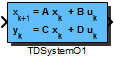
\includegraphics{TDSystemO1}\end{figure} 

\begin{XtoCtabular}{Inports}
In & Input \#1\tabularnewline
\hline
\end{XtoCtabular}


\begin{XtoCtabular}{Outports}
Out & Output \#1\tabularnewline
\hline
\end{XtoCtabular}

\begin{XtoCtabular}{Mask Parameters}
A & State matrix A\tabularnewline
\hline
B & Input matrix B\tabularnewline
\hline
C & Output matrix C\tabularnewline
\hline
D & Feedthrough matrix D\tabularnewline
\hline
\end{XtoCtabular}

\subsubsection*{Description:}
1st order time discrete system with one input and one output.

% include optional documentation file
\InputIfFileExists{\XcHomePath/Library/Control/Doc/TDSystemO1_Info.tex}{\vspace{1ex}}{}

\subsubsection*{Implementations:}
\begin{tabular}{l l}
\textbf{FiP8} & 8 Bit Fixed Point Implementation\tabularnewline
\textbf{FiP16} & 16 Bit Fixed Point Implementation\tabularnewline
\textbf{FiP32} & 32 Bit Fixed Point Implementation\tabularnewline
\textbf{Float32} & 32 Bit Floating Point Implementation\tabularnewline
\textbf{Float64} & 64 Bit Floating Point Implementation\tabularnewline
\end{tabular}

\XtoCImplementation{FiP8}
\index{Block ID!3344}
\nopagebreak[0]
% Implementation details
\begin{tabular}{l l}
\textbf{Name} & FiP8 \tabularnewline
\textbf{ID} & 3344 \tabularnewline
\textbf{Revision} & 1 \tabularnewline
\textbf{C filename} & TDSystemO1\_FiP8.c \tabularnewline
\textbf{H filename} & TDSystemO1\_FiP8.h \tabularnewline
\end{tabular}
\vspace{1ex}

8 Bit Fixed Point Implementation

\begin{XtoCtabular}{Controller Parameters}
a11 & Coefficient a11\tabularnewline
\hline
b11 & Coefficient b11\tabularnewline
\hline
c11 & Coefficient c11\tabularnewline
\hline
d11 & Coefficient d11\tabularnewline
\hline
sfra11 & Shift factor for coefficient a11\tabularnewline
\hline
sfrb11 & Shift factor for coefficient b11\tabularnewline
\hline
sfrc11 & Shift factor for coefficient c11\tabularnewline
\hline
sfrd11 & Shift factor for coefficient d11\tabularnewline
\hline
x1 & State x1\tabularnewline
\hline
\end{XtoCtabular}

% Implementation data structure
\XtoCDataStruct{Data Structure:}
\begin{lstlisting}
typedef struct {
     uint16        ID;
     int8          *In;
     int8          Out;
     int8          a11;
     int8          b11;
     int8          c11;
     int8          d11;
     uint8         sfra11;
     uint8         sfrb11;
     uint8         sfrc11;
     uint8         sfrd11;
     int8          x1;
} TDSYSTEMO1_FIP8;
\end{lstlisting}

\ifdefined \AddTestReports
\InputIfFileExists{\XcHomePath/Library/Control/Doc/Test_TDSystemO1_FiP8.tex}{}{}
\fi
\XtoCImplementation{FiP16}
\index{Block ID!3345}
\nopagebreak[0]
% Implementation details
\begin{tabular}{l l}
\textbf{Name} & FiP16 \tabularnewline
\textbf{ID} & 3345 \tabularnewline
\textbf{Revision} & 1 \tabularnewline
\textbf{C filename} & TDSystemO1\_FiP16.c \tabularnewline
\textbf{H filename} & TDSystemO1\_FiP16.h \tabularnewline
\end{tabular}
\vspace{1ex}

16 Bit Fixed Point Implementation

\begin{XtoCtabular}{Controller Parameters}
a11 & Coefficient a11\tabularnewline
\hline
b11 & Coefficient b11\tabularnewline
\hline
c11 & Coefficient c11\tabularnewline
\hline
d11 & Coefficient d11\tabularnewline
\hline
sfra11 & Shift factor for coefficient a11\tabularnewline
\hline
sfrb11 & Shift factor for coefficient b11\tabularnewline
\hline
sfrc11 & Shift factor for coefficient c11\tabularnewline
\hline
sfrd11 & Shift factor for coefficient d11\tabularnewline
\hline
x1 & State x1\tabularnewline
\hline
\end{XtoCtabular}

% Implementation data structure
\XtoCDataStruct{Data Structure:}
\begin{lstlisting}
typedef struct {
     uint16        ID;
     int16         *In;
     int16         Out;
     int16         a11;
     int16         b11;
     int16         c11;
     int16         d11;
     uint8         sfra11;
     uint8         sfrb11;
     uint8         sfrc11;
     uint8         sfrd11;
     int16         x1;
} TDSYSTEMO1_FIP16;
\end{lstlisting}

\ifdefined \AddTestReports
\InputIfFileExists{\XcHomePath/Library/Control/Doc/Test_TDSystemO1_FiP16.tex}{}{}
\fi
\XtoCImplementation{FiP32}
\index{Block ID!3346}
\nopagebreak[0]
% Implementation details
\begin{tabular}{l l}
\textbf{Name} & FiP32 \tabularnewline
\textbf{ID} & 3346 \tabularnewline
\textbf{Revision} & 1 \tabularnewline
\textbf{C filename} & TDSystemO1\_FiP32.c \tabularnewline
\textbf{H filename} & TDSystemO1\_FiP32.h \tabularnewline
\end{tabular}
\vspace{1ex}

32 Bit Fixed Point Implementation

\begin{XtoCtabular}{Controller Parameters}
a11 & Coefficient a11\tabularnewline
\hline
b11 & Coefficient b11\tabularnewline
\hline
c11 & Coefficient c11\tabularnewline
\hline
d11 & Coefficient d11\tabularnewline
\hline
sfra11 & Shift factor for coefficient a11\tabularnewline
\hline
sfrb11 & Shift factor for coefficient b11\tabularnewline
\hline
sfrc11 & Shift factor for coefficient c11\tabularnewline
\hline
sfrd11 & Shift factor for coefficient d11\tabularnewline
\hline
x1 & State x1\tabularnewline
\hline
\end{XtoCtabular}

% Implementation data structure
\XtoCDataStruct{Data Structure:}
\begin{lstlisting}
typedef struct {
     uint16        ID;
     int32         *In;
     int32         Out;
     int32         a11;
     int32         b11;
     int32         c11;
     int32         d11;
     uint8         sfra11;
     uint8         sfrb11;
     uint8         sfrc11;
     uint8         sfrd11;
     int32         x1;
} TDSYSTEMO1_FIP32;
\end{lstlisting}

\ifdefined \AddTestReports
\InputIfFileExists{\XcHomePath/Library/Control/Doc/Test_TDSystemO1_FiP32.tex}{}{}
\fi
\XtoCImplementation{Float32}
\index{Block ID!3347}
\nopagebreak[0]
% Implementation details
\begin{tabular}{l l}
\textbf{Name} & Float32 \tabularnewline
\textbf{ID} & 3347 \tabularnewline
\textbf{Revision} & 0.1 \tabularnewline
\textbf{C filename} & TDSystemO1\_Float32.c \tabularnewline
\textbf{H filename} & TDSystemO1\_Float32.h \tabularnewline
\end{tabular}
\vspace{1ex}

32 Bit Floating Point Implementation

\begin{XtoCtabular}{Controller Parameters}
a11 & Coefficient a11\tabularnewline
\hline
b11 & Coefficient b11\tabularnewline
\hline
c11 & Coefficient c11\tabularnewline
\hline
d11 & Coefficient d11\tabularnewline
\hline
x1 & State x1\tabularnewline
\hline
\end{XtoCtabular}

% Implementation data structure
\XtoCDataStruct{Data Structure:}
\begin{lstlisting}
typedef struct {
     uint16        ID;
     float32       *In;
     float32       Out;
     float32       a11;
     float32       b11;
     float32       c11;
     float32       d11;
     float32       x1;
} TDSYSTEMO1_FLOAT32;
\end{lstlisting}

\ifdefined \AddTestReports
\InputIfFileExists{\XcHomePath/Library/Control/Doc/Test_TDSystemO1_Float32.tex}{}{}
\fi
\XtoCImplementation{Float64}
\index{Block ID!3348}
\nopagebreak[0]
% Implementation details
\begin{tabular}{l l}
\textbf{Name} & Float64 \tabularnewline
\textbf{ID} & 3348 \tabularnewline
\textbf{Revision} & 0.1 \tabularnewline
\textbf{C filename} & TDSystemO1\_Float64.c \tabularnewline
\textbf{H filename} & TDSystemO1\_Float64.h \tabularnewline
\end{tabular}
\vspace{1ex}

64 Bit Floating Point Implementation

\begin{XtoCtabular}{Controller Parameters}
a11 & Coefficient a11\tabularnewline
\hline
b11 & Coefficient b11\tabularnewline
\hline
c11 & Coefficient c11\tabularnewline
\hline
d11 & Coefficient d11\tabularnewline
\hline
x1 & State x1\tabularnewline
\hline
\end{XtoCtabular}

% Implementation data structure
\XtoCDataStruct{Data Structure:}
\begin{lstlisting}
typedef struct {
     uint16        ID;
     float64       *In;
     float64       Out;
     float64       a11;
     float64       b11;
     float64       c11;
     float64       d11;
     float64       x1;
} TDSYSTEMO1_FLOAT64;
\end{lstlisting}

\ifdefined \AddTestReports
\InputIfFileExists{\XcHomePath/Library/Control/Doc/Test_TDSystemO1_Float64.tex}{}{}
\fi
